\chapter{Introducción.}\label{ch:introduccion}
\markboth{CAPÍTULO \ref{ch:introduccion}. INTRODUCCIÓN.}{}

En este primer capítulo de la memoria vamos a explicar las motivaciones que nos llevaron a pensar en realizar dicho proyecto, los objetivos que nos marcamos cuando lo diseñamos, los materiales usados y la organización de esta memoria.

\section{¿Por qué decidimos hacer el proyecto?}
Al igual que muchos estudiantes de la Universidad de Málaga, yo suelo hacer uso habitualmente del servicio de la cafetería en la facultad. A diario he observado que hay muchas personas que se molestan cuando les piden que cumplimenten y firmen el justificante que sirve a la universidad para el recuento de los estudiantes que comen diariamente en la cafetería, para pagar el posterior descuento por ser estudiante. Además de este inconveniente observé un par de problemas más, que son: lo molesto que es tener que firmar todos los días o habitualmente y la perdida de tiempo en las colas que se forman al rellenar el nombre y la firma. Por eso se decidió hacer una aplicación para terminales móviles con la que agilizar todo este proceso de firma y control de estudiantes, mediante la lectura de un código QR que tendría la información necesaria para la realización de la firma.

A medida que avanzaba el proyecto se vio que se podía ampliar la funcionalidad de la aplicación, no sólo al comedor, sino también a alquiler de pistas o cualquier documento necesario en la Universidad de Málaga.

Otra razón para la realización de este proyecto es que a mí me gusta la seguridad informática y vi en este proyecto una buena forma de aprender más sobre criptografía, particularmente en la criptografía de clave pública. También consideré que era un buen método para aprender a programar terminales Android, debido al gran auge que tienen en la actualidad, este tipo de terminales móviles, y a crear aplicaciones web de las que no tenía ninguna idea. Al inicio se pensó en hacerla directamente en Java sin ninguna ayuda, pero se descartó ante la dificultad de encontrar un servicio de hosting gratuito, por lo que se decidió cambiar ante una sugerencia que hizo el director de proyecto de usar una plataforma que proporciona Google llamada Google App Engine, que es gratuita y con la que se pueden crear aplicaciones web programadas en el lenguaje de programación Java y así tener la posibilidad de aprender otras APIS, no sólo Java2EE.

\section{Objetivos que queríamos conseguir.}

El principal objetivo que queríamos lograr era que la forma de firmar fuera de una forma muy fácil y que no fuera un mecanismo muy engorroso. Para ello decidimos realizar una aplicación para smartphone Android y una aplicación web para el almacenamiento y posterior comprobación de las firmas.

Una vez teníamos clara la idea, empezamos a diseñar un sistema con el que se pudiera realizar la firma digital, inicialmente sólo de un recibo inicialmente y finalmente ampliarlo a cualquier documento de la UMA, agilizando de esta forma dicho proceso.

%TODO: Hay poner algo de criptografía... xDDD

En la parte de la aplicación de Android se decidió hacer una aplicación clara y que fuese fácil de usar. Para eso usamos la API nivel 14 que equivale a la versión 4.0 de Android, llamada Ice Cream Sandwich. Se eligió, entre otras, porque dicha versión proporciona una nueva forma de diseño de las interfaces, un nuevo tema llamado Holo y muchas nuevas herramientas, como por ejemplo es el action bar, que es una barra que permanece siempre en la parte superior de la pantalla, la cual se va acomodando a las necesidades que tiene la aplicación cambiando los botones con diferentes funcionalidades, por ejemplo si estamos en la pantalla principal siempre tendremos siempre visible el botón de añadir un nuevo recibo que abrirá el lector de códigos QR (se puede observar en la primera barra de la figura~\ref{fig:actionBar}) sin embargo si estamos visualizando un recibo solo tendremos el botón de volver atrás, como se puede ver en la segunda barra de la figura~\ref{fig:actionBar}, en la que se puede ver que al lado del icono de la aplicación una flechita que indica que es el botón para volver atrás.

\begin{figure}
  \centering
    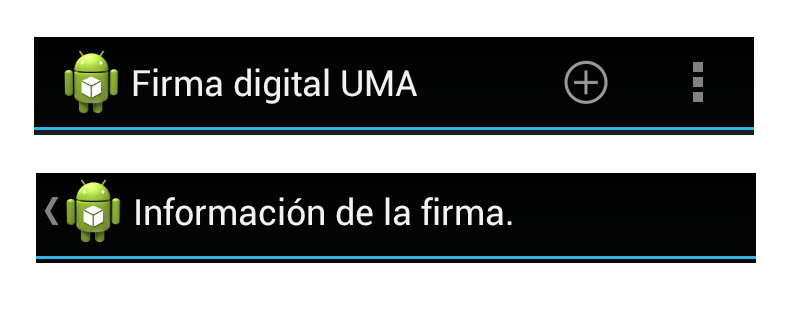
\includegraphics[scale=0.3]{./Introduccion/imagenes/actionbar.png}
  \caption{Action Bar.}
  \label{fig:actionBar}
\end{figure}

Al tomar la decisión de programar para terminales con Android 4.0 o mayor estuvimos sopesando los pros y los contras, y al final decidimos que la implantación de Android 4.0 cada vez es mayor y que cada día hay más terminales con dicha versión. Podemos ver en el gráfico de la figura~\ref{fig:graficoEvolucionAndroid} que a finales de octubre de este año la cantidad de usuarios que poseerían la versión 4.0 o mayor sería más del 15\% de terminales. En el gráfico de la figura~\ref{fig:graficoUsoAndroid} podemos ver que aunque todavía sigue reinando la versión 2.3.3, el cambio a la versión 4.0 o superior será rápida debido a todas las ventajas que aporta y mucho más ahora que hace unos meses Google sacó una nueva versión, la 4.1, llamada Jelly Bean, lo que va a obligar que casi todas las compañías quieran actualizar sus terminales a la última versión. Por lo que a pesar de dejar a un gran número de usuarios sin poder usar la aplicación inicialmente, preferimos funcionalidad y elegancia frente a gran cantidad de usuarios, ya que estos llegarán a medida que sus compañías actualicen sus terminales.


\begin{figure}
  \centering
    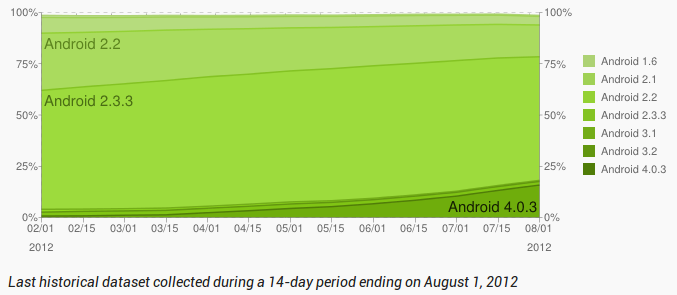
\includegraphics[scale=0.8]{./Introduccion/imagenes/graficoEvolucionAndroid.png}
  \caption{Gráfico de las versiones de Android a principio de octubre del 2012.}
  \label{fig:graficoEvolucionAndroid}
\end{figure}

\begin{figure}
  \centering
    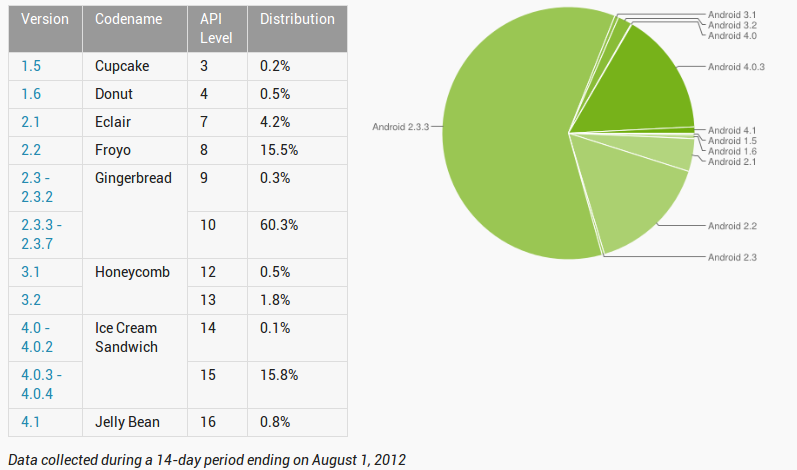
\includegraphics[scale=0.5]{./Introduccion/imagenes/graficoUsoAndroid.png}
  \caption{Gráfico del uso de las versiones de Android a principios de octubre del 2012.}
  \label{fig:graficoUsoAndroid}
\end{figure}

En la parte del servidor al elegir la plataforma de Google, hubo muchos elementos que resultaron muy fáciles a costa de tener que aprender a usar el SDK que Google proporciona, que como era una de las condiciones por la que elegimos dicha plataforma no nos importó. Una de las características que nos facilitaba es la gestión de usuarios, que los gestiona Google directamente al tener que usar una cuenta de Google Account para usar la aplicación web. Toda la seguridad y mantenimiento de los servidores, copias de seguridad, balanceos de carga y otra gran cantidad de funciones también las realiza Google, por lo que nos eximen de su realización y no tendremos que preocuparnos por ellas.

\section{Organización de la memoria.}

En este primer capítulo, hemos realizado una introducción al proyecto, los objetivos planteados y los materiales usados. Para continuar en el capítulo segundo de la memoria explicaremos los conocimientos básicos sobre todas las tecnologías usadas en el proyecto, como pueden ser Android, Java, criptografía, HTML, GIT, etc. Seguidamente, en el tercer capítulo hemos hecho una breve introducción a la criptografía que hemos usado a lo largo del proyecto, centrándonos más en la criptografía de clave pública, RSA y cómo usarla con el lenguaje de programación Java. Posteriormente, en el capítulo cuarto, exponemos los conocimientos básicos necesarios para entender Android y Google App Engine, explicamos los archivos que se usan en ambos proyectos y las características principales de cada arquitectura. Siguiendo con la memoria, en el capítulo quinto el principal de ella, se explica la arquitectura diseñada para el proyecto, la metodología usada y la implementación tanto de la aplicación móvil en Android como de ambas aplicaciones web. En el último capítulo tendremos el desenlace del proyecto en el que expondremos las conclusiones, problemas encontrados y posibles trabajos futuros que hemos observado que se podrían realizar. Para finalizar tendremos tres anexos en los que explicaremos la configuración de la plataforma Eclipse para el uso de la API Google App Engine como la de Android, la creación de los certificados de clave pública y el contenido del CD. Al final podemos encontrar el índice general, el índice de figuras y la bibliografía usada.

\section{Material usado.}
Para la realización del proyecto hemos usado un ordenador personal para todo el proceso de programación y un smartphone con Android para la depuración y prueba de la aplicación. 

El ordenador es un ordenador portátil, con Ubuntu 12.04 como sistema operativo, un procesador Pentium Dual Core a 2.2Ghz, 4 Gb de memoria RAM.

El móvil usado es un Samsung Galaxy Nexus (figura~\ref{fig:nexus}) que fue el móvil presentado cuando Google lanzó la versión 4.0, por lo que es también el primer terminal en usar Android 4.0 y meses después el primero en recibir la actualización de Android 4.1. Sus características son una pantalla de 4.65 pulgadas Super Amoled con resolución de 1280 x 720, procesador Dual-Core a 1.2Ghz, HSPA+, NFC, Wifi, GPS, etc.

\begin{figure}
  \centering
    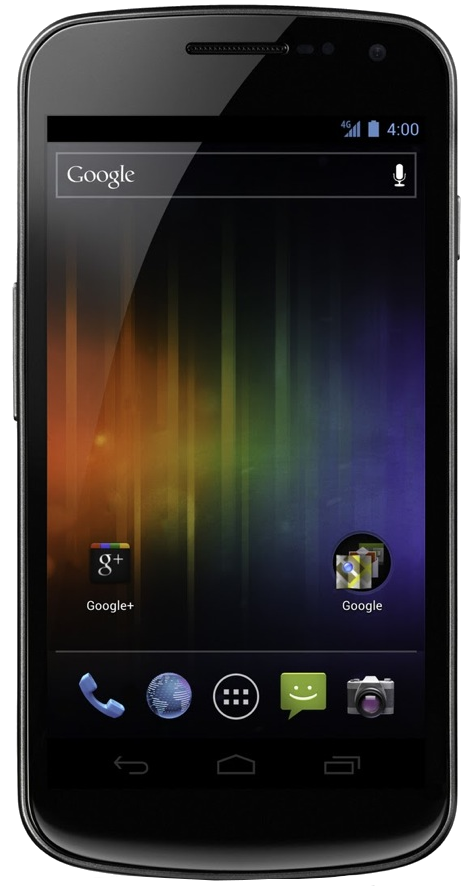
\includegraphics[scale=0.3]{./Introduccion/imagenes/nexus.png}
  \caption{Samsung Galaxy Nexus.}
  \label{fig:nexus}
\end{figure}

No tenemos datos sobre las máquinas usadas por los servidores donde Google da el servicio de Google App Engine.

